\documentclass[12pt]{article}
\usepackage{amsmath, amssymb, amsthm}
\usepackage{mathtools}
\usepackage{graphicx}
\usepackage{float}
\usepackage{xcolor}
\usepackage{listings}
\usepackage{geometry}
\usepackage{algorithm}
\usepackage{algpseudocode}
\usepackage{tikz}
\usepackage{longtable}
\usepackage{circuitikz}
\usepackage{comment}
\usepackage{MnSymbol}
\usepackage{physics}
\usepackage{booktabs}
\usepackage[section]{placeins}
\usepackage[colorlinks=true, urlcolor=blue, linkcolor=red]{hyperref}

\providecommand{\brak}[1]{\ensuremath{\left(#1\right)}}

\title{}
\author{EE24BTECH11002 Agamjot Singh\\IIT Hyderabad}
\date{\today}

\begin{document}
%\maketitle

\section*{Task 3 - Power Management System}
Okay first things first, what do we have to build?\\
It's basically just a robotic arm that can move around.

\subsection*{What do we have?}
Let's see what we're working with.

\begin{table}[h]
\centering
\begin{tabular}{ll}
\toprule
\textbf{Components} & \textbf{Quantity} \\
\midrule
Brushed DC Geared Motors & 4 \\
BLDC Motors & 2 \\
Servo Motors & 3 \\
NEMA Stepper Motor & 1 \\
Raspberry Pi 5 & 1 \\
RPI Camera Module 3 & 1 \\
Ldrobot D500 LiDAR Kit & 1 \\
ESP32 & 1 \\
\bottomrule
\end{tabular}
\end{table}

\subsection*{Our objective}
\begin{itemize}
\item Schematic - Basically what goes where
\item Appropriate Battery Selection
\item Safety Features (including a kill switch of course)
\item Power Distribution Analysis 
\end{itemize}

\newpage

\subsection*{Schematic - What goes where}
\subsubsection*{Motor Specifications}
We first focusing on the Torque specifications of all the motors to figure what motors to use in locomotion vs the robotic arm itself.
\begin{table}[h]
\centering
\begin{tabular}{lll}
\toprule
\textbf{Components} & \textbf{Quantity} & \textbf{Rated Torque} \\
\midrule
Brushed DC Motors & 4 & 11 kg-cm \\
BLDC Motors & 2 & 0.573 kg-cm \\
Servo Motors & 3 & 28.8 to 35 kg-cm \\
NEMA Stepper Motor (2 Phase) & 1 & 2.9 kg-cm \\
\bottomrule
\end{tabular}
\end{table}
\FloatBarrier

Calculating that rated torque for the ECO II Series 2207 BLDC Motor was not that straightforward.

The torque of a BLDC motor can be calculated using the formula,
\begin{equation*}
\text{Torque} = K_t \times \text{Current}
\end{equation*}

where $K_t$ is the torque constant, which is related to the kV rating.

First, we convert the kV rating from RPM/Volt to the SI unit rad/s/Volt,

\begin{align*}
K_v(\text{SI}) &= 1700 \times \frac{2\pi}{60} \text{ rad/s/V} \\
K_v(\text{SI}) &= 177.89 \text{ rad/s/V}
\end{align*}

The torque constant $K_t$ is the reciprocal of $K_v$ in SI units,

\begin{align*}
K_t = \frac{1}{K_v(\text{SI})} &= \frac{1}{177.89} = 0.00562 \text{ Nm/A}\\
\text{Rated Torque} &= K_t \times \text{Rated Current} \\
\text{Rated Torque} &= 0.00562 \text{ Nm/A} \times 10 \text{ A} \\
\text{Rated Torque} &= 0.0562 \text{ Nm} = 0.0562 \text{ kg-cm}
\end{align*}

\subsubsection*{Motor Selection}
\textbf{Locomotion:} An obvious choice for the locomotion would be the 4 Brushed DC Geared Motors which provide enough torque for the load movement and is pretty suitable in a 4-wheel drive configuration.
\newline
If we were to choose some other motor, say the servo motor because of its much higher torque, then we would have to make a tricycle drive which is certainly not suitable for high loads and stability.

\textbf{Base joint actuator:} The base motor has to overcome the frictional force and in addition, has to handle the angular acceleration of the whole robotic arm.
\begin{align}
    \tau_{\text{base}} = \tau_{\text{friction}} + I\alpha
\end{align}
where $I$ is the moment of inertia and $\alpha$ is the angular acceleration at that instant about the axis.
\newline
Assuming we'll keep $\alpha$ minimal and proper lubrication of the motors (avoiding $\tau_{\text{friction}}$), the torque required is quite minimal. On the other hand the precision required is massive which can only be provided by the NEMA Stepper motor. Lesser torque but the precision, boosted by software microstepping, is more suited to the base motor.

\textbf{Shoulder joint actuator:} Here we define some terminologies. Let the Load mass be $m$, link lengths be $L_1, L_2, L_3$, link masses be $M_1, M_2, M_3$, end effector mass be $M_0$ (including the motors for the end effector). This will be clearer to the reader by the figure below. The actuators themselves have masses $A_1, A_2, A_3$ and $A_0$ as the end effector.
\newline
Coming back to the shoulder joint actuator $A_1$, the maximum torque required is quite huge. It can be calculated by taking into account the maximum extension case.

\begin{multline*}
    \tau_{\text{shoulder}} = \frac{M_1 g L_1}{2} + A_2 g L_1 + M_2 g \brak{L_1 + \frac{L_2}{2}} + A_3 g \brak{L_1 + L_2} + \\ M_3 g \brak{L_1 + L_2 + \frac{L_3}{2}} + A_0 g \brak{L_1 + L_2 + L_3}
\end{multline*}

This is quite a huge quantity (the most torque in this whole project in fact) and can only be supported by a servo motor. The choice we make for the shoulder joint is the Pro-Range OT5330M Servo motor.

\textbf{Elbow joint actuator:} 
For the elbow joint actuator $A_2$, the maximum torque in maximum extension case is given by,
\begin{multline*}
    \tau_{\text{elbow}} = M_2 g \brak{L_1 + \frac{L_2}{2}} + A_3 g \brak{L_1 + L_2} + \\ M_3 g \brak{L_1 + L_2 + \frac{L_3}{2}} + A_0 g \brak{L_1 + L_2 + L_3}
\end{multline*}

This is lesser than the torque required in case of the shoulder joint actuator but it is still a huge quantity and can also only be supported by a servo motor. The choice we make for the elbow joint is also the Pro-Range OT5330M Servo motor.

\textbf{Wrist joint actuator:} 
For the wrist joint actuator $A_3$, the maximum torque in maximum extension case is given by,
\begin{align*}
    \tau_{\text{wrist}} = M_3 g \brak{L_1 + L_2 + \frac{L_3}{2}} + A_0 g \brak{L_1 + L_2 + L_3}
\end{align*}

This is lesser than the torque required in case of the shoulder and elbow joint actuator but it is still a higher quantity and can also only be supported by a servo motor. The choice we make for the wrist joint is also the Pro-Range OT5330M Servo motor.

\textbf{End effector actuators:} These actuators dont need $\textit{that}$ much torque as the other joints but have to be more versatile. We may need to use it as a gripper or say as a drill-ish machine which require precision/speed at once. Considering this and also the fact that the only motors which are left are the BLDC motors, we're just gonna use the ECO II Series 2207 BLDC Motors.

\subsubsection*{Motor Controllers and Drivers}
First off, our motor controller choice is pretty obvious. It's the ESP32 microcontroller. Because of its computation restrictions we can't really use it as the main driver with the object detection with lidars and camera on it, but motor driving signals are easy to compute.
\newline
On top of this, motor drivers for all the motors except the servos (which don't really require a driver) are a necessity. The schematic explaining what im talking about is given below. The COMMS go to Raspberry Pi.

\begin{figure}[!ht]
\centering
\resizebox{1\textwidth}{!}{%
\begin{circuitikz}
\tikzstyle{every node}=[font=\small]
\draw  (3.75,11) rectangle (5.25,9.25);
\draw  (7,13.25) rectangle (8.75,10.25);
\draw  (10,12) rectangle (11,11.25);
\draw  (12.5,12) rectangle (13.5,11.25);
\draw  (13.75,12) rectangle (14.75,11.25);
\draw  (11.25,12) rectangle (12.25,11.25);
\draw  (7,9.75) rectangle (8.75,8);
\draw  (11.5,9.75) rectangle (12.75,9);
\draw  (10,9.75) rectangle (11.25,9);
\draw  (10,7.5) rectangle (11,6.75);
\draw  (11.25,7.5) rectangle (12.25,6.75);
\draw  (12.5,7.5) rectangle (13.5,6.75);
\draw (5.25,10.75) to[short] (7,10.75);
\draw (5.25,10.5) to[short] (6.5,10.5);
\draw (6.5,10.5) to[short] (6.5,9.25);
\draw (6.5,9.25) to[short] (7,9.25);
\draw (5.25,10.25) to[short] (6.25,10.25);
\draw (6.25,10.25) to[short] (6.25,7);
\draw (6.25,7) to[short] (10,7);
\draw (11.75,6.75) to[short] (11.75,6.25);
\draw (11.75,6.25) to[short] (6,6.25);
\draw (6,6.25) to[short] (6,10);
\draw (6,10) to[short] (5.25,10);
\draw (5.25,9.75) to[short] (5.75,9.75);
\draw (5.75,9.75) to[short] (5.75,6);
\draw (5.75,6) to[short] (13,6);
\draw (13,6.75) to[short] (13,6);
\node [font=\small] at (10.5,7.25) {Servo};
\node [font=\small] at (11.75,7.25) {Servo};
\node [font=\small] at (13,7.25) {Servo};
\node [font=\small] at (10.6,9.5) {BLDC};
\node [font=\small] at (12.1,9.5) {BLDC};

\draw  (13,9.75) rectangle (14.55,9); % Stepper
\node [font=\small] at (13.75,9.5) {Stepper};
\draw (13.75,9) to[short] (13.75,8.25);
\draw (13.75,8.25) to[short] (8.75,8.25);

\node [font=\normalsize] at (10.5,11.75) {DC};
\node [font=\normalsize] at (11.75,11.75) {DC};
\node [font=\normalsize] at (13,11.75) {DC};
\node [font=\normalsize] at (14.25,11.75) {DC};
\draw (8.75,11.5) to[short] (10,11.5);
\draw (8.75,9.25) to[short] (10,9.25);
\draw (12,9) to[short] (12,8.5); % --
\draw (12,8.5) to[short] (8.75,8.5);
\draw (8.75,12.5) to[short] (11.75,12.5);
\draw (11.75,12.5) to[short] (11.75,12);
\draw (13,11.25) to[short] (13,10.75);
\draw (13,10.75) to[short] (8.75,10.75);
\draw (8.75,13) to[short] (14.25,13);
\draw (14.25,13) to[short] (14.25,12);
\node [font=\normalsize] at (4.5,10.25) {ESP32};
\node [font=\normalsize] at (7.75,12.75) {Motor};
\node [font=\normalsize] at (7.75,12.25) {Driver};
\node [font=\normalsize] at (7.75,9.25) {Motor};
\node [font=\normalsize] at (7.75,8.75) {Driver};
\node [font=\small] at (3.55,13.25) {COMMS};
\draw [ dashed] (9.75,13.25) rectangle  (15,10.5);
\node [font=\small] at (10.6,13.5) {Navigation};
\draw [ dashed] (9.75,10) rectangle  (15,5.75);
\node [font=\small] at (10.25,5.5) {Arm};
\draw [<->, >=Stealth] (4.5,15.5) -- (4.5,11);
\draw  (3.5,17) rectangle (5.75,15.5);
\node [font=\large] at (4.5,16.25) {RPI};
\draw (5.75,16.75) to[short] (8,16.75);
\draw (5.75,15.75) to[short] (8,15.75);
\draw  (8,17) rectangle (10.5,16.25);
\draw  (8,16) rectangle (10.5,15.25);
\node [font=\small] at (9.25,16.6) {LiDAR};
\node [font=\small] at (9.25,15.6) {Camera};
\draw (7.75,14.5) to[short] (7.75,13.25);
\draw (7.75,14.5) to[short] (12.75,14.5);
\draw (7.75,10.25) to[short] (7.75,9.75);
\draw (12.75,15.25) to[short] (12.75,14.5);
\draw  (12,16.75) rectangle (15.25,15.25);
\node [font=\normalsize] at (13.55,16) {Battery Pack};
\end{circuitikz}
}%

\label{fig:my_label}
\caption{Overview Schematic}
\end{figure}
\FloatBarrier

\subsubsection*{Battery Pack}
The battery pack consists not merely the battery but the safety and protection systems in place to avoid, well, catastrophes. In place is a \textbf{BMS} (Battery management system), \textbf{Fuse} to avoid short circuits, \textbf{Fool's diode} to prevent reverse current, and a \textbf{Master Kill Switch} for turning off the whole bot. The battery pack schematic is given below.

\begin{figure}[!ht]
\centering
\resizebox{1\textwidth}{!}{%
\begin{circuitikz}
\tikzstyle{every node}=[font=\small]
\draw  (3.75,11) rectangle (6.25,9.75);
\draw (5,12.5) to[short] (5,11);
\draw (5,9.75) to[short] (5,8.25);
\draw (5,12.5) to[short] (9.75,12.5);
\draw (9.75,12.5) to[normal open switch] (11.75,12.5);
\node at (10.5,12.5) [circ] {};
\node at (11,12.5) [circ] {};
\node at (11.75,12.5) [circ] {};
\node at (9.75,12.5) [circ] {};
\draw  (7.5,11) rectangle (10,9.75);
\draw (5,11.75) to[short] (7.75,11.75);
\draw (7.75,11.75) to[short] (7.75,11);
\draw (5,9) to[short] (7.75,9);
\draw (7.75,9.75) to[short] (7.75,9);
\draw (9.75,11.75) to[L ] (11.75,11.75);
\draw (9.75,11.75) to[short] (9.75,11);
\draw (11.75,11.75) to[short] (11.75,10.25);
\draw (11.75,10.25) to[short] (10,10.25);
\draw (8.25,9.75) to[short] (8.25,8.25);
\draw  (8.75,8.75) rectangle (11.25,7.75);
\draw (5,8.25) to[short] (8.75,8.25);
\draw (11.25,8.25) to[short] (17.25,8.25);
\draw (11.75,12.5) to[short] (13.25,12.5);
\draw (9,9.75) to[short] (9,9.25);
\draw (9,9.25) to[short] (12,9.25);
\draw (12,9.25) to[short] (12,8.25);
\draw  (13.25,12.75) rectangle (15,12);
\draw (15,12.5) to[short] (17.25,12.5);
\draw (16,8.25) to[empty Schottky diode] (16,12.5);
\draw (5,8.25) to (5,7.75) node[ground]{};
\draw [->, >=Stealth, dashed] (8.75,11) -- (8.75,14.25);
\node [font=\small] at (5.25,11.25) {+};
\node [font=\small] at (5.25,9.5) {-};
\node [font=\small] at (17.5,12.5) {+};
\node [font=\small] at (17.5,8.25) {-};
\node [font=\normalsize] at (5,10.4) {Battery};
\node [font=\normalsize] at (8.75,10.35) {BMS};
\node [font=\normalsize] at (14.1,12.4) {Fuse};
\node [font=\small] at (10,8.5) {Current};
\node [font=\small] at (10,8.15) {Sensor};
\draw [ dashed] (3.5,13.25) rectangle  (17,7);
\node [font=\normalsize] at (5,13.5) {Battery pack};
\end{circuitikz}
}%

\label{fig:my_label}
\end{figure}
\FloatBarrier

The Fool's diode will help in case of reverse currents as all the reverse current will flow through the diode instead of the actual load. We are gonna use a Schottky diode for this purpose due to its high reverse bias breakdown voltage (about 50 to 60 V which is more than enough).
\newline
What battery are we gonna choose? Well we haven't calculated the power specifications yet (which will we will do somewhere down the line), but one thing's sure. It's going to be around 12 V nominal voltage battery (or we could stoop down do 11.1 V if we like 3S LiPo Batteries).

\subsubsection*{Powering the RPI and ESP32 - Voltage Regulators}
Since we're using a 12 V battery, it will blow up our Raspberry Pi and ESP32 instantly. We obviously don't want that, so we use voltage regulators which in this case, we will be using a \textbf{Buck Converter} to bring down the voltage to 5V for the RPI, ESP32, LiDAR and Camera Modules. In addition to that, we would also need a 7.4 V power line for the Servo motors to optimally run them for which will be using a different buck converter.

\begin{figure}[!ht]
\centering
\resizebox{1\textwidth}{!}{%
\begin{circuitikz}
\tikzstyle{every node}=[font=\small]
\draw  (3.75,11) rectangle (5.25,9.25);
\draw  (7,13.25) rectangle (8.75,10.25);
\draw  (10,12) rectangle (11,11.25);
\draw  (12.5,12) rectangle (13.5,11.25);
\draw  (13.75,12) rectangle (14.75,11.25);
\draw  (11.25,12) rectangle (12.25,11.25);
\draw  (7,9.75) rectangle (8.75,8);
\draw  (11.5,9.75) rectangle (12.75,9);
\draw  (10,9.75) rectangle (11.25,9);
\draw  (10,7.5) rectangle (11,6.75);
\draw  (11.25,7.5) rectangle (12.25,6.75);
\draw  (12.5,7.5) rectangle (13.5,6.75);
\draw (5.25,10.75) to[short] (7,10.75);
\draw (5.25,10.5) to[short] (6.5,10.5);
\draw (6.5,10.5) to[short] (6.5,9.25);
\draw (6.5,9.25) to[short] (7,9.25);
\draw (5.25,10.25) to[short] (6.25,10.25);
\draw (6.25,10.25) to[short] (6.25,7);
\draw (6.25,7) to[short] (10,7);
\draw (11.75,6.75) to[short] (11.75,6.25);
\draw (11.75,6.25) to[short] (6,6.25);
\draw (6,6.25) to[short] (6,10);
\draw (6,10) to[short] (5.25,10);
\draw (5.25,9.75) to[short] (5.75,9.75);
\draw (5.75,9.75) to[short] (5.75,6);
\draw (5.75,6) to[short] (13,6);
\draw (13,6.75) to[short] (13,6);

\draw  (13,9.75) rectangle (14.55,9); % Stepper
\node [font=\small] at (13.75,9.5) {Stepper};
\draw (13.75,9) to[short] (13.75,8.25);
\draw (13.75,8.25) to[short] (8.75,8.25);

\node [font=\small] at (10.5,7.25) {Servo};
\node [font=\small] at (11.75,7.25) {Servo};
\node [font=\small] at (13,7.25) {Servo};
\node [font=\small] at (10.6,9.5) {BLDC};
\node [font=\small] at (12.1,9.5) {BLDC};
\node [font=\normalsize] at (10.5,11.75) {DC};
\node [font=\normalsize] at (11.75,11.75) {DC};
\node [font=\normalsize] at (13,11.75) {DC};
\node [font=\normalsize] at (14.25,11.75) {DC};
\draw (8.75,11.5) to[short] (10,11.5);
\draw (8.75,9.25) to[short] (10,9.25);
\draw (12,9) to[short] (12,8.5);
\draw (12,8.5) to[short] (8.75,8.5);
\draw (8.75,12.5) to[short] (11.75,12.5);
\draw (11.75,12.5) to[short] (11.75,12);
\draw (13,11.25) to[short] (13,10.75);
\draw (13,10.75) to[short] (8.75,10.75);
\draw (8.75,13) to[short] (14.25,13);
\draw (14.25,13) to[short] (14.25,12);
\node [font=\normalsize] at (4.5,10.25) {ESP32};
\node [font=\normalsize] at (7.75,12.75) {Motor};
\node [font=\normalsize] at (7.75,12.25) {Driver};
\node [font=\normalsize] at (7.75,9.25) {Motor};
\node [font=\normalsize] at (7.75,8.75) {Driver};
\node [font=\small] at (3.65,13.25) {COMMS};
\draw [ dashed] (9.75,13.25) rectangle  (15,10.5);
\node [font=\small] at (10.5,13.5) {Navigation};
\draw [ dashed] (9.75,10) rectangle  (15,5.75);
\node [font=\small] at (10.25,5.5) {Arm};
\draw [<->, >=Stealth] (4.5,15.5) -- (4.5,11);
\draw  (3.5,17) rectangle (5.75,15.5);
\node [font=\large] at (4.5,16.25) {RPI};
\draw (5.75,16.75) to[short] (8,16.75);
\draw (5.75,15.75) to[short] (8,15.75);
\draw  (8,17) rectangle (10.5,16.25);
\draw  (8,16) rectangle (10.5,15.25);
\node [font=\small] at (9.25,16.6) {LiDAR};
\node [font=\small] at (9.25,15.6) {Camera};
\draw (7.75,14.5) to[short] (7.75,13.25);
\draw (7.75,14.5) to[short] (12.75,14.5);
\draw (7.75,10.25) to[short] (7.75,9.75);
\draw (12.75,15.25) to[short] (12.75,14.5);
\draw  (12,16.75) rectangle (15.25,15.25);
\node [font=\normalsize] at (13.35,16) {Battery Pack};
\node [font=\small] at (10.25,14.75) {12 V};
\draw (12,18.25) to[short] (2.5,18.25);
\draw (2.5,18.25) to[short] (2.5,10.25);
\draw (2.5,10.25) to[short] (3.75,10.25);
\draw (2.5,16.5) to[short] (3.5,16.5);
\node [font=\small] at (10.25,18.5) {5 V};
\draw (10.5,8) to[short] (10.5,7.5);
\draw (10.5,8) to[short] (16.25,8);
\draw (11.75,8) to[short] (11.75,7.5);
\draw (13,8) to[short] (13,7.5);
\draw  (12,18.75) rectangle (15.25,17.5);
\draw (12.75,17.5) to[short] (12.75,16.75);
\node [font=\small] at (13.45,18.1) {Buck Converter};
\draw  (15.75,16.5) rectangle (17.75,14.25);
\node [font=\small] at (16.75,15.75) {Buck};
\draw (15.25,15.75) to[short] (15.75,15.75);
\draw (16.25,14.25) to[short] (16.25,8);
\node [font=\small] at (16.75,15.25) {Converter};
\node [font=\small] at (16.85,13.5) {7.4 V};
\end{circuitikz}
}%

\label{fig:my_label}
\caption{Final Schematic}
\end{figure}
\FloatBarrier

\subsection*{Power Distribution and Component Selection}
What are the extra components we need?
\begin{enumerate}
    \item Motor Drivers for 4$\times$ DC Motors and 2$\times$ BLDC Motors
    \item Variable Buck Converters (2$\times$)
    \item Battery
    \item BMS Chip
    \item Current Sensor
    \item Fuse
    \item Schottky Diode
    \item Master switch
\end{enumerate}

Okay firstly, we have to calculate the rough power consumption estimate.

\begin{table}[h]
\centering
\begin{tabular}{|l|c|c|c|}
\hline
\textbf{Component} & \textbf{Quantity} & \textbf{Rated Voltage (V)} & \textbf{Stall Current (A)} \\
\hline
DC Geared Motor (IG45) & 4 & 12.0 & 15.0 \\
\hline
BLDC (ECO II 2207) & 2 & 11.1-22.2 & 36.0 \\
\hline
NEMA Stepper (39HY38-0504) & 1 & 12.0 & 0.5 $\times$ 2 = 1 \\
\hline
Servo Motor (OT5330M) & 3 & 4.0-8.4 & 3.8 \\
\hline
Raspberry Pi 5 & 1 & 5.0 & 2.2 \\
\hline
Raspberry Pi Camera Module 3 & 1 & 5.0 & 0.25 \\
\hline
Ldrobot D500 LiDAR Kit & 1 & 5.0 & 0.29 \\
\hline
ESP32 & 1 & 5.0 & 0.3 \\
\hline
\end{tabular}
    \caption{Component Specifications}
\end{table}

\begin{table}[h]
\centering
\begin{tabular}{|l|c|c|c|}
\hline
\textbf{Component} & \textbf{Quantity} & \textbf{Operating Voltage (V)} & \textbf{Stall Power (W)} \\
\hline
DC Geared Motor (IG45) & 4 & 11.1 & 166.5 \\
\hline
BLDC (ECO II 2207) & 2 & 11.1 & 399.6 \\
\hline
NEMA Stepper (39HY38-0504) & 1 & 11.1 & 11.1 \\
\hline
Servo Motor (OT5330M) & 3 & 7.4 & 28.1 \\
\hline
Raspberry Pi 5 & 1 & 5.0 & 11.0 \\
\hline
Raspberry Pi Camera Module 3 & 1 & 5.0 & 1.25 \\
\hline
Ldrobot D500 LiDAR Kit & 1 & 5.0 & 1.45 \\
\hline
ESP32 & 1 & 5.0 & 1.5 \\
\hline
\end{tabular}
\caption{Power Requirements}
\end{table}

\begin{align*}
\text{DC Geared Motors (4x)} &= 4 \times 11.1\text{ V} \times 15.0\text{ A} = 666.0\text{ W} \\
\text{BLDC Motors (2x)} &= 2 \times 11.1\text{ V} \times 36.0\text{ A} = 799.2\text{ W} \\
\text{NEMA Stepper Motor (1x)} &= 1 \times 11.1\text{ V} \times 1\text{ A} = 11.1\text{ W} \\
\text{Servo Motors (3x)} &= 3 \times 4.0\text{ V} \times 3.8\text{ A} = 45.6\text{ W} \\
\text{Raspberry Pi 5} &= 5.0\text{ V} \times 2.2\text{ A} = 11.0\text{ W} \\
\text{Raspberry Pi Camera Module 3} &= 5.0\text{ V} \times 0.25\text{ A} = 1.25\text{ W} \\
\text{Ldrobot D500 LiDAR Kit} &= 5.0\text{ V} \times 0.29\text{ A} = 1.45\text{ W} \\
\text{ESP32} &= 5.0\text{ V} \times 0.3\text{ A} = 1.5\text{ W} \\
\textbf{Total Power} &= 1537.1\text{ W}
\end{align*}

That's a HUGE amount of power. Also you may notice that we have been taking 11.1 V as the operating voltage when the rated voltage was 12 V. That's because a 3s LiPo Battery has a nominal voltage of 11.1 V and peak voltage of 12.6 V, and these are the batteries we'll be using in this bot.
\newline
This rough power estimation has not taken into account the power consumed by motor drivers, the BMS, etc. has not been considered. Although they will be extremely less compared to the massive 1537 W of power.
\begin{align*}
    \textbf{Rough Current Drawn} = 1537.1/11.1 = 138.47\text{ A}
\end{align*}
Now this will affect all the materials we choose henceforth.

\subsubsection*{Battery}
The battery we're going for is a Pro-Range 11.1V 5200mAh 40C 3S Lithium Polymer Battery Pack. 
\newline
This pack has a three cell series combination which results in 11.1 V of voltage and a capacity of 5200mAh along with 40 C as the C rating.
\begin{align*}
    \text{Max continous discharge current} &= \text{(capacity)}\times\text{(C rating)}\\
    &= 5200 \times 40 = 208000\text{ mA}\\
    &= 208\text{ A}
\end{align*}

So this has an headroom of about 70 A which is MORE than enough. The cost of this battery is about 3653 rupees.

\href{https://robu.in/product/pro-range-5200mah-3s-40c80c-lithium-polymer-battery-pack-lipo/}{Link for the component can be found here.}


\subsubsection*{Fuse}
The fuse we selected is LittelFuse Auto 200A 58VDC Fuse. This also has a headroom of about 60 A above the max discharge current. This costs about 377 rupees.

\href{https://www.digikey.in/en/products/detail/littelfuse-inc/142.5631.6202/2515909?gad_source=1&gad_campaignid=20498599563&gbraid=0AAAAADrbLljJD7EDQKu9e9nLQij0boGQ3&gclid=CjwKCAjw_pDBBhBMEiwAmY02NlW6MqK-9fe1ue4tsHIFhOGmYJwIuewU8G1YjnB5rM2lacEHPa4Z9hoCnioQAvD_BwE&gclsrc=aw.ds}{Link for the component can be found here.}

\subsubsection*{Schottky Diode}
We're going for an extremely cheap but useful SS34 Schottky Diode. This costs about 25 rupees.

\href{https://robu.in/product/ss34-schottky-diode-for-high-speed-switching-pack-of-2/?gad_source=1&gad_campaignid=17427802703&gbraid=0AAAAADvLFWebM7-G2QsFY7UCdjSACyQJK&gclid=CjwKCAjw_pDBBhBMEiwAmY02Ng7v65L4U7x7HYcmHqhfgriCHJnP5DWrVZJornA1QMzXB2dP9AnKdRoC5OUQAvD_BwE}{Link for the component can be found here.}

\subsubsection*{Master/Kill Switch}
This switch will be in the form of a relay, because it also has to be controlled by the BMS systems. We need a relay that can handle atleast 12V DC at 150 A. Unfortunately these types of relays are pretty hard to find, and are on the expensive side.
\newline
We're going to be using the 12V 200A Car Start Relay which costs about 1493 rupees.

\href{https://order2india.com/products/12v-200a-car-start-relay-with-accessories?variant=43710190583930&utm_source=google&utm_medium=organic&utm_campaign=ALL&utm_content=12V\%20200A\%20Car\%20Start\%20Relay\%20with\%20Accessories&gad_source=1&gad_campaignid=21058867647&gbraid=0AAAAADjpDzQd_h_QiVlT-siNAMC-BX8IV&gclid=CjwKCAjw_pDBBhBMEiwAmY02NoSwFztjR-UFZ8ERJ-SUvc4wo6-MO1Tyu-ZFE0xYVFXtt13ZgQBkBhoCj_MQAvD_BwE}{Link for the component can be found here.}

\subsubsection*{BMS}
The BMS for our current specifications, 3S LiPo with atleast 150 A of max discharge was EXTREMELY hard to find. Hate to say it, but I had to set up a proxy server to access AliExpress. I found a 3S 150A Battery Protection Board Balance MOS High Current BMS. 
This costs about 1557 rupees.

Usually BMS barely take in any current, so because of lack of proper datasheets for this BMS, we're gonna assume it takes in negligible amount of current and hence consumes pretty less power (relatively).

\href{https://www.aliexpress.com/item/1005003684963240.html}{Link for the component can be found here.}

\begin{figure}
    \begin{center}
        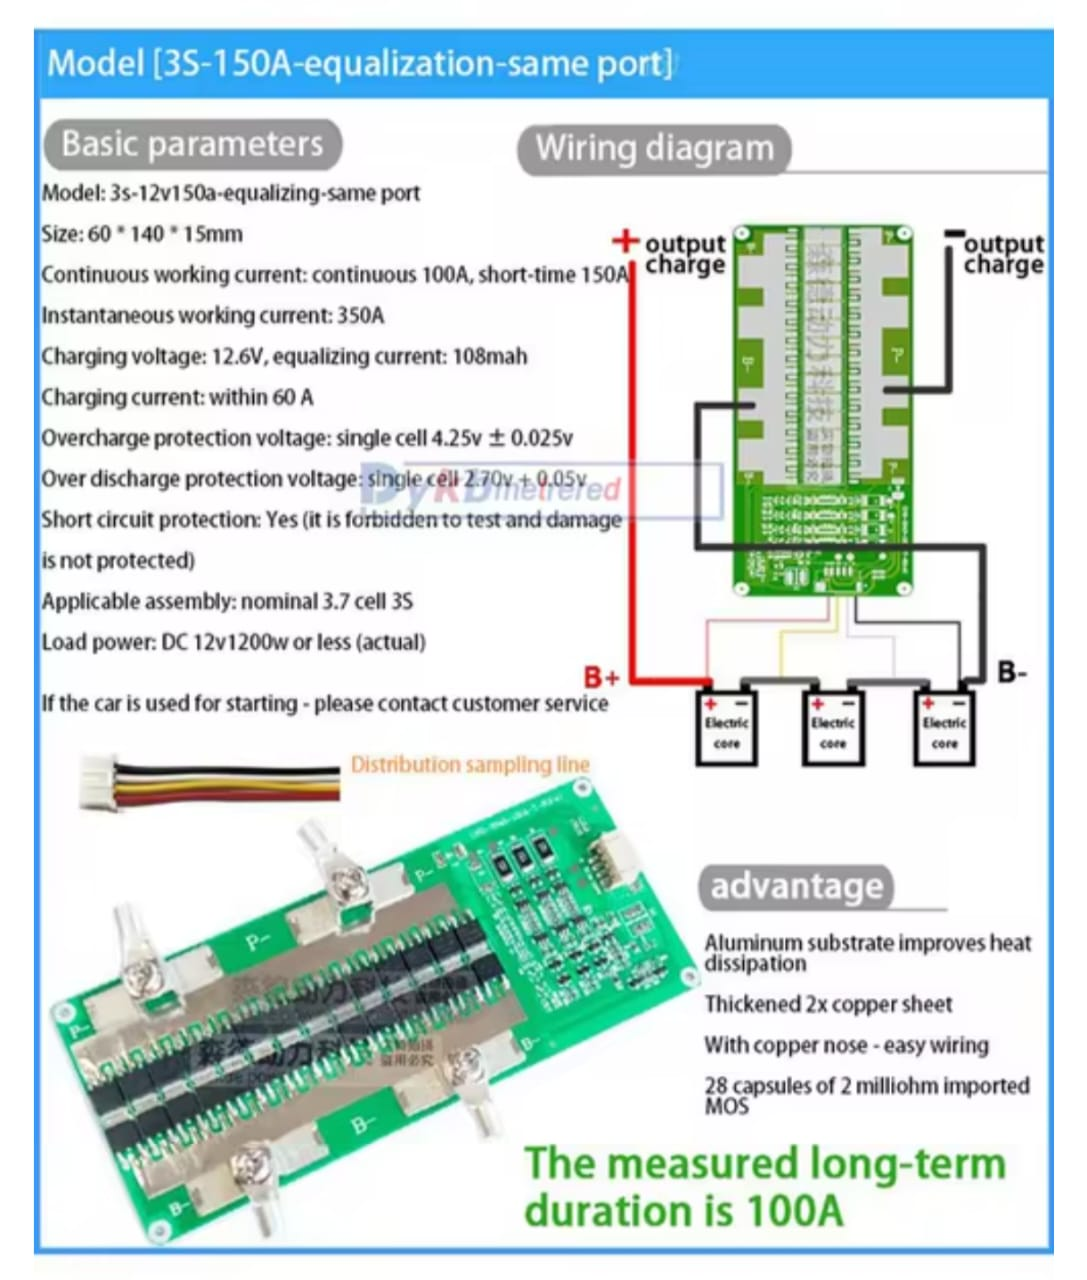
\includegraphics[width=0.75\textwidth]{bms.jpeg}
    \end{center}
    \caption{Data supplied by the vendor}\label{fig:}
\end{figure}
\FloatBarrier


\begin{figure}[!ht]
\centering
\resizebox{1\textwidth}{!}{%
\begin{circuitikz}
\tikzstyle{every node}=[font=\small]
\draw  (3.75,11) rectangle (5.25,9.25);
\draw  (7,13.25) rectangle (8.75,10.25);
\draw  (10,12) rectangle (11,11.25);
\draw  (12.5,12) rectangle (13.5,11.25);
\draw  (13.75,12) rectangle (14.75,11.25);
\draw  (11.25,12) rectangle (12.25,11.25);
\draw  (7,9.75) rectangle (8.75,8);
\draw  (11.5,9.75) rectangle (12.75,9);
\draw  (10,9.75) rectangle (11.25,9);
\draw  (10,7.5) rectangle (11,6.75);
\draw  (11.25,7.5) rectangle (12.25,6.75);
\draw  (12.5,7.5) rectangle (13.5,6.75);
\draw (5.25,10.75) to[short] (7,10.75);
\draw (5.25,10.5) to[short] (6.5,10.5);
\draw (6.5,10.5) to[short] (6.5,9.25);
\draw (6.5,9.25) to[short] (7,9.25);
\draw (5.25,10.25) to[short] (6.25,10.25);
\draw (6.25,10.25) to[short] (6.25,7);
\draw (6.25,7) to[short] (10,7);
\draw (11.75,6.75) to[short] (11.75,6.25);
\draw (11.75,6.25) to[short] (6,6.25);
\draw (6,6.25) to[short] (6,10);
\draw (6,10) to[short] (5.25,10);
\draw (5.25,9.75) to[short] (5.75,9.75);
\draw (5.75,9.75) to[short] (5.75,6);
\draw (5.75,6) to[short] (13,6);
\draw (13,6.75) to[short] (13,6);
\node [font=\small] at (10.5,7.25) {Servo};
\node [font=\small] at (11.75,7.25) {Servo};
\node [font=\small] at (13,7.25) {Servo};
\node [font=\small] at (10.5,9.5) {BLDC};
\node [font=\small] at (12,9.5) {BLDC};
\node [font=\normalsize] at (10.5,11.75) {DC};
\node [font=\normalsize] at (11.75,11.75) {DC};
\node [font=\normalsize] at (13,11.75) {DC};
\node [font=\normalsize] at (14.25,11.75) {DC};
\draw (8.75,11.5) to[short] (10,11.5);
\draw (8.75,9.25) to[short] (10,9.25);
\draw (12,9) to[short] (12,8.5);
\draw (12,8.5) to[short] (8.75,8.5);
\draw (8.75,12.5) to[short] (11.75,12.5);
\draw (11.75,12.5) to[short] (11.75,12);
\draw (13,11.25) to[short] (13,10.75);
\draw (13,10.75) to[short] (8.75,10.75);
\draw (8.75,13) to[short] (14.25,13);
\draw (14.25,13) to[short] (14.25,12);
\node [font=\normalsize] at (4.5,10.25) {ESP32};
\node [font=\normalsize] at (7.75,12.75) {Motor};
\node [font=\normalsize] at (7.75,12.25) {Driver};
\node [font=\normalsize] at (7.75,9.25) {Motor};
\node [font=\normalsize] at (7.75,8.75) {Driver};
\node [font=\small] at (3.75,13.25) {COMMS};
\draw [ dashed] (9.75,13.25) rectangle  (15,10.5);
\node [font=\small] at (10.5,13.5) {Navigation};
\draw [ dashed] (9.75,10) rectangle  (15,5.75);
\node [font=\small] at (10.25,5.5) {Arm};
\draw [<->, >=Stealth] (4.5,15.5) -- (4.5,11);
\draw  (3.5,17) rectangle (5.75,15.5);
\node [font=\large] at (4.5,16.25) {RPI};
\draw (5.75,16.75) to[short] (8,16.75);
\draw (5.75,15.75) to[short] (8,15.75);
\draw  (8,17) rectangle (10.5,16.25);
\draw  (8,16) rectangle (10.5,15.25);
\node [font=\small] at (9.25,16.5) {LiDAR};
\node [font=\small] at (9.25,15.5) {Camera Module};
\draw (7.75,14.5) to[short] (7.75,13.25);
\draw (7.75,14.5) to[short] (12.75,14.5);
\draw (7.75,10.25) to[short] (7.75,9.75);
\draw (12.75,15.25) to[short] (12.75,14.5);
\draw  (12,16.75) rectangle (15.25,15.25);
\node [font=\normalsize] at (13.25,16) {Battery Pack};
\node [font=\small] at (10.25,14.75) {11.1 V};
\draw (12,18.25) to[short] (2.5,18.25);
\draw (2.5,18.25) to[short] (2.5,10.25);
\draw (2.5,10.25) to[short] (3.75,10.25);
\draw (2.5,16.5) to[short] (3.5,16.5);
\node [font=\small] at (10.25,18.5) {5 V};
\draw (10.5,8) to[short] (10.5,7.5);
\draw (10.5,8) to[short] (16.25,8);
\draw (11.75,8) to[short] (11.75,7.5);
\draw (13,8) to[short] (13,7.5);
\draw  (12,18.75) rectangle (15.25,17.5);
\draw (12.75,17.5) to[short] (12.75,16.75);
\node [font=\small] at (13.25,18) {Buck Converter};
\draw  (15.75,16.5) rectangle (17.75,14.25);
\node [font=\small] at (16.75,15.75) {Buck};
\draw (15.25,15.75) to[short] (15.75,15.75);
\draw (16.25,14.25) to[short] (16.25,8);
\node [font=\small] at (16.75,15.25) {Converter};
\node [font=\small] at (16.75,13.5) {7.4 V};
\node [font=\small] at (6.75,17) {290 mA};
\node [font=\small] at (6.75,16) {250 mA};
\node [font=\small] at (6.75,15.5) {5 V};
\node [font=\small] at (6.75,16.5) {5 V};
\node [font=\small] at (3,16.75) {2.2 A};
\node [font=\small] at (3,16.25) {5V};
\node [font=\small] at (3,10.5) {0.3 A};
\node [font=\small] at (3,10) {5 V};
\node [font=\small, rotate around={-90:(0,0)}] at (14,12.5) {11.1V};
\node [font=\small, rotate around={-90:(0,0)}] at (14.5,12.5) {15 A};
\node [font=\small] at (11.5,8.75) {11.1V};
\node [font=\small] at (10.5,8.75) {36A};
\node [font=\small] at (13.5,7.75) {7.4 V};
\node [font=\small] at (12.5,7.75) {3.8 A};
\draw  (13,9.75) rectangle (14.75,9);
\node [font=\small] at (13.75,9.5) {Stepper};
\draw (8.75,8.25) to[short] (13.75,8.25);
\draw (13.75,8.25) to[short] (13.75,9);
\node [font=\small] at (14.25,8.5) {11.1V};
\node [font=\small] at (13.25,8.5) {1A};
\end{circuitikz}
}%

\label{fig:my_label}
\end{figure}












\end{document}
